\documentclass{article}

\usepackage{graphicx, pslatex, array}
\usepackage[table]{xcolor}

\widowpenalty=1000
\clubpenalty=1000

\pagestyle{plain}

\setlength{\parindent}{0pt}%
\setlength{\parskip}{\baselineskip}%
\setlength{\oddsidemargin}{0in}
\setlength{\textwidth}{6.5in}
\setlength{\textheight}{8.5in}
\newlength\acklength
\newlength\logowidth
\setlength\logowidth{1.8in}

\setlength{\arrayrulewidth}{1.5pt}

\newcommand{\cubed}{$^3$}
\newcommand{\micro}{\ensuremath{\mu}}
\newcommand{\fc}{\cellcolor{salmon}}
\newcommand{\nfc}{\cellcolor{white}}
\definecolor{salmon}{rgb}{1.0,0.8,0.7}
\newcommand{\highlightbox}[1]{\colorbox{salmon}{\parbox{\linewidth}{#1}}}

\hyphenation{Neutralization}
\hyphenation{Orleans}

% Allow this template to be latex'd directly.
% Can't just say \newcommand{\ subst} because that confuses templater.
\expandafter\newcommand\csname subst\endcsname[1]{{\bf #1}}

\newcommand{\inunits}        {\subst{inunits}} 
\newcommand{\outunits}       {\subst{outunits}} 
\newcommand{\longinunits}    {\subst{longinunits}} 
\newcommand{\longoutunits}   {\subst{longoutunits}} 
\newcommand{\sampleinfo}     {\subst{sampleinfo}} 
\newcommand{\user}           {\subst{user}}

\begin{document}

\title{Levels of Concern Report \\
       \large
       A comparison of air sample results to levels of concern}
\author{\user}
\date{}
\maketitle

\section*{Sample information}
\begin{itemize}
\sampleinfo
\item Report date:               \today
\item Report input units:        \longinunits\ (\inunits)$^*$
\item Report output units:       \longoutunits\ (\outunits)$^*$
\item Report made on web at:     http://myairsample.org
\end{itemize}

\newcommand{\unitsnote}{
$^*$For a description of what units mean, see ``Units Information'' section later in this report
}

\subst{unitsnote}

\newcommand{\unitssection}{
\section*{Units information}
Parts per billion (ppb) describes how many parts of a chemical are in
the same place as 1 billion parts of air. For example, a recipe says
to add a spoonful of vanilla for every 10 cups of flour. A drop of
vanilla is hardly anything, but it has a big effect on the cookies'
flavor. Similarly, if we measure benzene in the air, we might find 3
``drops'' of benzene for 1,000,000,000 (one billion) ``drops'' of air. Three
drops of benzene seems like a small amount, but it is significant.

Parts per billion by volume, or ppbv, means the concentration has been
figured out in terms of how much space the molecules take up. For
example, if we make a mixture of 3 cups of vanilla and 1 billion cups
of flour, then our concentration is 3 parts volume (cups of vanilla)
per billion parts volume (cups of flour), or 3 ppbv vanilla in
flour. When 3 volumes of benzene are in a billion volumes of air, the
concentration is 3 ppbv benzene in air.

Micrograms per meters cubed (\micro g/m\cubed) describes how much of a chemical's
weight is in a volume of air that takes up one cubic meter. Imagine an empty
box that is three feet long on both sides, and three feet tall. One meter is about
three feet long. So the box's volume is 1 cubic meter, or 1 m\cubed. A microgram
(\micro g) is a very small weight, like that of a grain of sand. You put 3 grains of sand
into the box. The concentration of sand inside the box is the weight of the sand
(3 \micro g) divided by the
volume of the box (1 m\cubed), or 3 \micro g /m\cubed. Like grains of sand, chemicals can also be
reported by weight and volume. For example, a monitor might read 5 \micro g /m\cubed\ %
benzene, or 5 \micro g of benzene in 1 m\cubed\ of air.
}

\newcommand{\standardssection}{
\section*{Sample screening levels}

\highlightbox{Some government agencies have developed standards and screening levels for
toxic chemicals in the air based on health information about the chemicals.
There is no information available for some toxic chemicals. The agencies are
listed below, with a brief description of the methods used in establishing their
levels. States may not be required to adhere to national standards.}

\begin{itemize}
\subst{standardblurbs}
\end{itemize}

}

     \vfill
     \parbox{\logowidth}{
       \includegraphics[width=\logowidth]{labb_logo}\\
       \vskip 0.1in
       
\includegraphics[width=\logowidth]{drcs_logo-200}\\
       \vskip 0.1in
       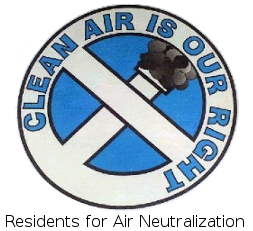
\includegraphics[width=\logowidth]{RANlogo-text}
     }
     \setlength\acklength{\textwidth}
     \addtolength\acklength{-\logowidth}
     \addtolength\acklength{-0.7in}
     \hskip 0.5in
     \parbox{\acklength}{
       \sloppy
       This report was generated at www.myairsample.org, a site
       \linebreak
       developed and maintained by the Louisiana Bucket Brigade,
       \linebreak
       Residents for Air Neutralization, and Digitial Resources for
       \linebreak
       Community and Science.  For questions and comments about air
       data, Louisiana Bucket Brigade can contacted at
       www.labucketbrigade.org, 4226 Canal St, New Orleans, LA 70119,
       phone: 504-484-3433, fax: 504-324-0332, email:
       info@labucketbrigade.org.  For comments, feedback, or errors in
       the web site, please contact the LA Bucket Brigade or email
       Digital Resources for Community and Science at
       drcsdirector@gmail.com
     }

\thispagestyle{empty}

\subst{resultssection}

Note: For any EPA Region 6 Screening Levels reported here, the
www.myairsample.org tool that generated this report used levels from
when the tool was originally developed in $\sim$2003.  Most of the EPA
Region 6 Screening Levels appear to have changed since then.  The
following levels of concern in the tool were updated in March 2014:
ATSDR Minimal Risk Levels, Louisiana Ambient Air Quality Standards,
North Carolina Ambient Air Standards, and Texas Effects Screening
Levels - any of these levels in the report are up-to-date as of March
2014.

\subst{unitssection}
\subst{standardssection}

\end{document}

